%% Default Latex document template
%%
%%  blake@rcs.ee.washington.edu

\documentclass[letterpaper]{article}

% Uncomment for bibliog.
%\bibliographystyle{unsrt}

\usepackage{graphicx}
\usepackage{lineno}
\usepackage{amsmath}

%\usepackage{fancyhdr}

%%%%%%%%%%%%%%%%%%%%%%%%%%%%%%%%%%%%%%%%5
%
%  Set Up Margins

%%%%%%%%%%%%%%%%%%%%%%%%%%%%%%%%%%%%%%%%%%%%%%%%%
% include file for:
%      Critical Page setup dimensions
%            DO NOT MODIFY
%       (for help see "Latex Line by Line" p 260)
%
\setlength\oddsidemargin{0in}
\setlength\evensidemargin{0in}

\usepackage[left=0.98in, right=0.98in, top=1.0in, bottom=1.0in]{geometry}

% %Top Margin and header
% \setlength\voffset{-0.94in}
% \setlength\topmargin{0.25in}
% \setlength\headheight{0.25in}
% %\setlength\headwidth{6.5in}
% \setlength\headsep{0.25in}
% %Body
% \setlength\textwidth{6.5in}
% \setlength\textheight{9.50in}
% %Footer
% %\setlength\footheight{0.5in}
% \setlength\footskip{0.3750in}
% Line spacing for 6 lines per inch
\linespread{0.894}  % 1.0 = single    1.6 = double
%
%          END of Critical Page Setup Dimensions
%%%%%%%%%%%%%%%%%%%%%%%%%%%%%%%%%%%%%%%%%%%%%%%%%%%

%%%%%%%%%%%%%%%%%%%%%%%%%%%%%%%%%%%%%%%%%%%%%%%%%%%
%
% Useful style and math macros
%


\newcommand\Dfrac[2]{\frac{\displaystyle #1}{\displaystyle #2}}
\newcommand\beq{\begin{equation}}
\newcommand\eeq{\end{equation}}

\newcommand\bmat{\begin{bmatrix}}
\newcommand\emat{\end{bmatrix}}

\newenvironment{solution}
{\ttfamily \vspace{0.155in} {\bf SOLUTION:} \\ }
{ \vspace{0.25in} \par }



%
%        Font selection
%
%\renewcommand{\rmdefault}{ptm}             % Times
%\renewcommand{\rmdefault}{phv}             % Helvetica
%\renewcommand{\rmdefault}{pcr}             % Courier
%\renewcommand{\rmdefault}{pbk}             % Bookman
%\renewcommand{\rmdefault}{pag}             % Avant Garde
%\renewcommand{\rmdefault}{ppl}             % Palatino
%\renewcommand{\rmdefault}{pch}             % Charter


%%%%%%%%%%%%%%%%%%%%%%%%%%%%%%%%%%%%%%%%%%%%%%%%%
%
%         Page format Mods HERE
%
%Mod's to page size for this document
\addtolength\textwidth{0cm}
\addtolength\oddsidemargin{0cm}
\addtolength\headsep{0cm}
\addtolength\textheight{0cm}
%\linespread{0.894}   % 0.894 = 6 lines per inch, 1 = "single",  1.6 = "double"

% header options for fancyhdr

%\pagestyle{fancy}
%\lhead{LEFT HEADER}
%\chead{CENTER HEADER}
%\rhead{RIGHT HEADER}
%\lfoot{Hannaford, U. of Washington}
%\rfoot{\today}
%\cfoot{\thepage}



% Make table rows deeper
%\renewcommand\arraystretch{2.0}% Vertical Row size, 1.0 is for standard spacing)

\begin{document}
\begin{centering}
{\Large   Simulation of Everting Tube Experiments}

Blake Hannaford

\today

\end{centering}

\section{Introduction}
The dynamic model of an eversion drive system includes;
\begin{itemize}
  \item An everting tube of length $L$ and growth rate $\dot{L}$.
  \item A pressurized housing
  \item A reel with rotation $\theta, \dot{\theta}, \ddot{\theta}$, on which tubing is rolled having inertia (assume fixed) of
  $J$ and radius $r$.
  \item A brake which applies a Coulomb friction torque to the reel
  \[
    \tau_c = C\mathrm{sgn}(\dot{\theta})
  \]
  \item A ``crumple zone" in which eversion material can accumulate
  between the reel and the everting tube. The length of material in
  the crumple zone is $L_c$.
  \item Eversion happens when the eversion force (pressure $\times$ face area of the tube) exceeds any retarding forces.
  \item Forces which can oppose eversion include,
  \begin{itemize}
    \item drag forces inertial forces required to pull the tubing material
    inside the deployed tube,
    \item reel inertia and reel friction resulting from unspooling material,
  \end{itemize}
\end{itemize}

\noindent
The everting tube can be in one of two states:
\begin{itemize}
  \item GROWING (the tube is actively everting, $\dot{L}>0$)
  \item STUCK (the tube is not growing due to insufficient everting force, $\dot{L}=0$)
\end{itemize}
and the reel/crumple zone can be in one of two additional states:

\begin{itemize}
  \item TAUGHT (the crumple zone has zero length , $L_c = 0 $)
  \item SLACK (there is material in the crumple zone, $L_c > 0$)
\end{itemize}

Together the system can be in four states comprising the permutations
of these two state variables.

\section{System Equations:}

After setting initial conditions (see below), we model eversion dynamics by:
\begin{enumerate}
  \item Computing pressure, volume, and flow from the source.
  \item Computing forces applied to the eversion tip.
  \item Accounting for the mechanical advantage (everting material speed is $2\times\dot{L}$, Pressure applied to everting front develops 1/2 the everting force expected from $P\times A$.)

  \item Selecting the dynamic mode from the four combined states above.
  GROWING and STUCK are selected by force thresholds applied to net
  eversion force.    TAUGHT and SLACK are selected by checking length of
  the crumple zone material.

  \item According to the dynamic mode, summing forces, equating to  zero, solving for tube and reel accelerations.
  \item Eversion does not come to an instant halt. We  empirically model exponential decay of velocity as tube decelerates.
\end{enumerate}

\noindent
Specifically:

%     # Eq 5.1
%     Fcoulomb = Tau_coulomb / rReel\_SIu
%     F_c.append(Fcoulomb)
%
%     # Eq 5.2
%     #Fdrag = L * Kdrag * 2.0 * Ldot  # material speed is 2x Ldot
%     F_d.append(Fdrag(L,Ldot))
%     F_j.append(Lddot*J/rReel\_SIu**2)

\begin{equation}\label{eqOneCompartmentVol}
V_t = V_{housing} - V_{contents} + L  A
\end{equation}
$V_t$ includes both the reel housing minus the volume of its contents,
and the everted tube of length $L$ with cross sectional area $A$.

From the ideal gas equation:
\begin{equation}\label{eqOneCompartmentPress}
P = \frac{N  R  T}{ V_t}
\end{equation}
where $N$ is the molar mass of gas in the system, $R$ is the gas constant, and $T$ is the temperature
in $^\circ$K, (which we assume is constant).

\begin{figure}\centering
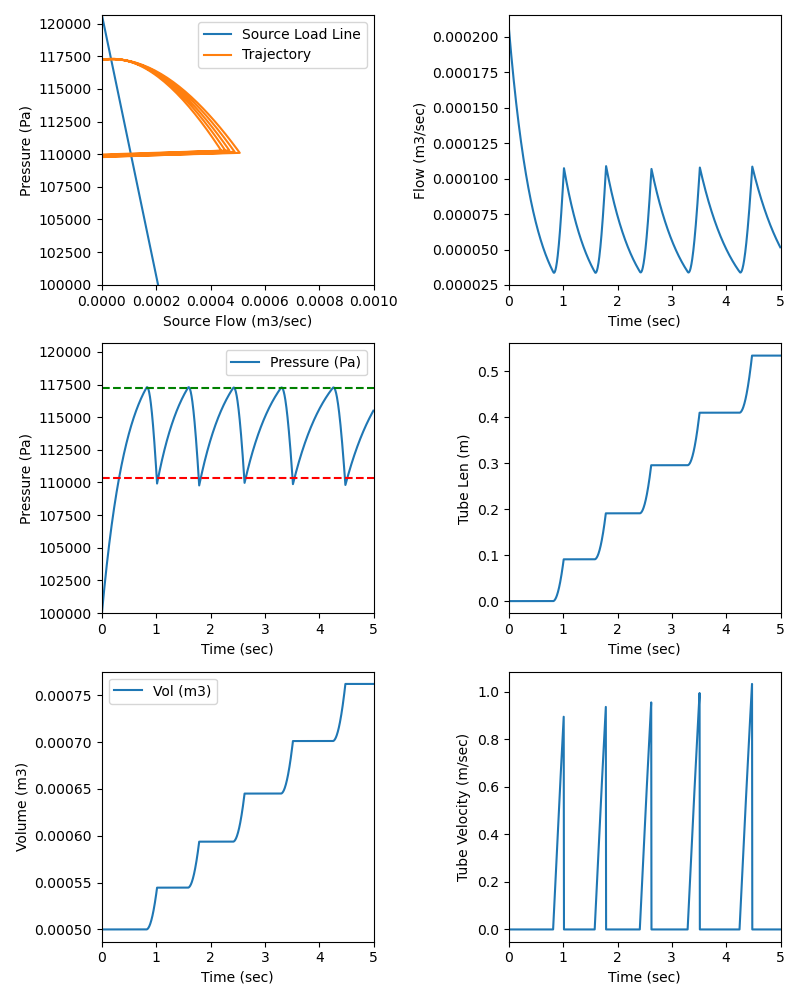
\includegraphics[width=.75\textwidth]{Figure_9HhiI_hiTf_baseline.png}
\caption{Simulation Run with approximate qualitative match.  (See Lewis, Fig 9, hiI, hiTf)}
\label{Fig:baselineResults}
\end{figure}

Computing Forces:


\begin{equation}
  F_{ever} = \mathrm{max}(0, PA/2)
\end{equation}
\beq
  F_{c} = \tau_{Coulomb} / r
\eeq

Coulomb friction is independent of velocity so does not get scaled by the $2\times$ mechanical advantage.

Computing acceleration according to the dynamic state:

GROWING and SLACK:

\beq
\ddot{L} = \frac{F_{ever} - F_D(L,\dot{L})-F_C}  {M_T}
\eeq
\beq
\dot{\theta} = \tau_{Coulomb}/J
\eeq

GROWING and TAUGHT:

%         Lddot = (1/Mt + (rReel\_SIu**2/J) ) * ( F_ever - Fdrag(L,Ldot) - Fcoulomb )
%         th_ddot = Lddot/rReel\_SIu
\beq
\ddot{L} =(F_{ever} - F_D - F_C) /  (M_T + J/r^2)
\eeq

\beq
\ddot{\theta} = \ddot{L}/r
\eeq

STUCK and (SLACK or TAUGHT):


%         alpha = 2000 * dt  # empirical fit
%         Lddot = -1 * max(0, alpha * Ldot)
%         th_ddot = tau_coulomb/J

\beq
\ddot{L} = -1 * \mathrm(max)(0, \alpha * \dot{L})
\eeq

\beq
\ddot{\theta} = \tau_{Coulomb} / J
\eeq
where $\alpha$ is an empirical time constant modeling the dynamics of eversion stopping.

Modeling flow from the pressure source (Thevenin equivalent):
\begin{equation}\label{eqOneCompartmentflow}
Fl_{source} = \frac {P_{source}-P} {R_{source}}
\end{equation}

Converting airflow ($m^3/sec$) to rate of molar mass flow:
\begin{equation}
\dot{N} = Fl_{source} \cdot \mathrm{moles\_per\_m3}
\end{equation}

Model velocity and length dependent eversion force which is resistance to pulling out eversion material:
\begin{equation}
F_D(L,\dot{L} = 2 L  K_D  \dot{L}
\end{equation}

Where the factor of two accounts for everting material going at twice tube growth rate, $\dot{L}$.

Update length of  crumpled material (if any)
\beq
L_C = \mathrm{max}(0,  r\theta - L)
\eeq

We have a switching model to replicate observed intermittent starting and stopping of eversion
which updates the state based on current pressure:
\begin{equation}
    \mathtt{state} =
    \begin{cases}
      \mathrm{GROWING}, &  P > P2 \\
      \mathrm{unchanged}, & P1 <= P <= P2 \\
      \mathrm{STUCK},   &  P < P1
    \end{cases}
\end{equation}



We are currently investigating changing this switching model to one based on thresholding
net eversion force rather than tip surface pressure:
\begin{equation}
    \mathtt{state1} =
    \begin{cases}
      \mathrm{GROWING},   &  F_{ever} > F2 \\
      \mathrm{unchanged}, &  F1 <= F_{ever} <= F2 \\
      \mathrm{STUCK},     &  F_{ever} < F1
    \end{cases}
\end{equation}

In either case above, we update the crumple state as
\begin{equation}
    \mathtt{state2} =
    \begin{cases}
      \mathrm{TAUGHT},  &  L_C <=0 \\
      \mathrm{SLACK},   &  L_C  > 0
    \end{cases}
\end{equation}

Finally, we integrate the state variables:
\begin{equation}
\begin{aligned}
  \dot{L} &= \dot{L} +  \ddot{L}  dt \\
  L       &= L + \dot{L}  dt \\
  \dot{\theta} &= \dot{\theta} + \ddot{\theta}dt \\
  \theta &= \theta + \dot{\theta} dt\\
  N &= N + \dot{N}  dt\\
\end{aligned}
\end{equation}


\subsection{Initial Conditions}
\begin{equation}
\begin{aligned}
  P &= 1 \; \mathrm{atmosphere}\\
  {\tt state1} &= STUCK \\
  {\tt state2} &= TAUGHT \\
  N &= N(V_{housing} - V_{contents}) / RT \\
  L &= 0\\
  \dot{L} &= 0\\
  \ddot{L} &= 0\\
\end{aligned}
\end{equation}

\section{Simulation Results}



\section{Simplified Simulation Results}
{\bf These initial results are from a simplified model assuming the TAUGHT state at all times. }
All parameters for the above model were computed from measurements of the experimental
system with the exception of {\tt PBA\_static, PHalt\_dyn, Kdrag} which were estimated
by a visual match to experimental data.
Initial simulation results using the baseline parameters (Sec. \ref{baselineParms}, below) are
given in Figure \ref{Fig:baselineResults}.

Some parameters were iteratively changed based on remaining observed differences
between Figure \ref{Fig:baselineResults} and experiment. Specifically:

\vspace{0.175in}
% \begin{table}[]
\begin{tabular}{p{1.5in}|l|l|l}
Observation       & Param    & Original Value & Modified Value      \\\hline
Velocities too high  & ${\tt Kdrag}$  &   0.3     & 0.6          \\\hline
Pressure thresholds converge with time& {\tt PBA\_static} & $1.17\times10^5 $Pa & $1.17\times10^5 - 500L$ Pa          \\\hline
Pressure thresholds converge with time & {\tt PHalt\_dyn} & $1.17\times10^5 $Pa & $1.013\times10^5 + 500L$ Pa       \\\hline
Pressure rise too slow  & $V_{housing}$   &  $0.5\times10^{-3}$ m$^3$   & $0.05\times10^{-3} $ m$^3$   \\\hline
Peak Velocity too high  & $J$             &  $5.10\times10^4$  kg/m$^2$     & 10.2$\times10^4$  kg/m$^2$ \\\hline
\end{tabular}
% \end{table}

\vspace{0.175in}

The modified parameter set is given in Section \ref{modParams} below.  Asterisks (*) denote iteratively changed parameters.

Simulation with the modified parameters (Figure \ref{Fig:ModifParResults}) improve the model fit to data by
    1) Shrinking loops on the pressure flow plot (upper left) are similar
  to shrinking loops in experimental pressure-velocity plot'
    2) Convergence of the eversion thresholds (center left) causes the shrinking loops above,
    3) Peak velocities better match peaks of fig. 9, and match the pattern of the highest velocity
  appearing near the center of travel.
    4) With the modified parmeters there are about 2 bursts per second, similar to the experimental rate.



\begin{figure}\centering
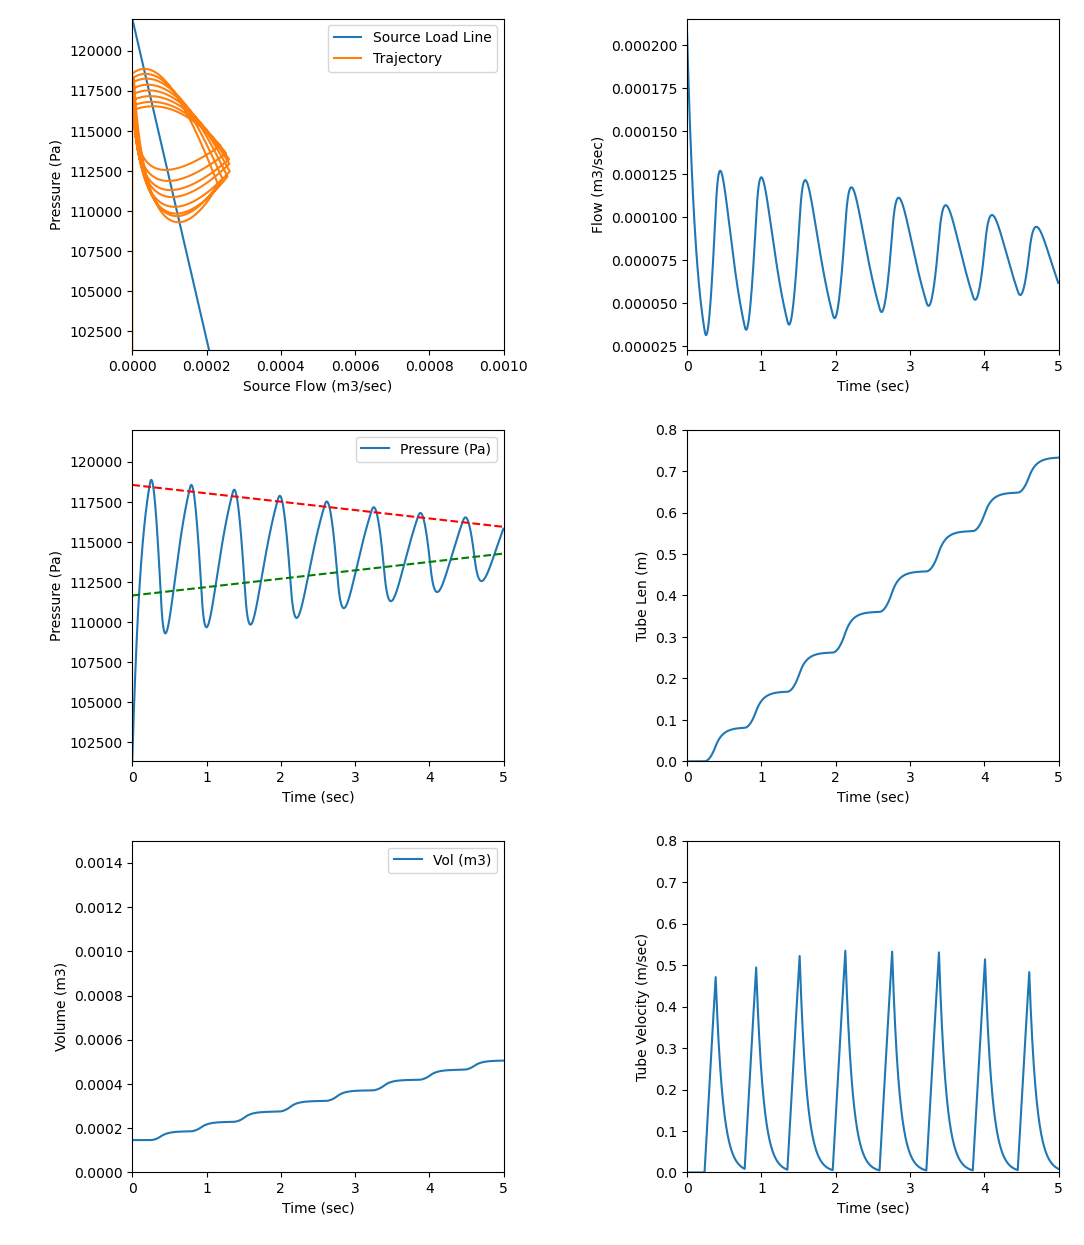
\includegraphics[width=.75\textwidth]{Figure_9HhiI_hiTf_tweakedParams.png}
\caption{Improved qualitative match with modified parameters.  (See Lewis, Fig 9, hiI, hiTf)}
\label{Fig:ModifParResults}
\end{figure}

\clearpage

\section{Baseline Parameter Values}\label{baselineParms}
\begin{verbatim}

      moles_per_m3   4.4623E+01  moles / m3
      Psource\_SIu    1.2066E+05  Pascals
      LLine\_SIu      1.0000E-08  m3/sec / Pascal
      Rsource\_SIu    1.0000E+08  Pa/m3/sec
      Vhousing_m3    1.4616E-03  m3
      Kdrag          3.0000E-01  N / m2 / sec
      area_m2        4.9087E-04  m2
      Pintercept     1.2066E+05  Pascals
      Fintercept     2.0684E-04  m3/sec
      Vintercept     4.2137E-01  m/sec
      PBA_static     1.1721E+05  Pascals
      PHalt_dyn      1.1032E+05  Pascals
      Patmosphere    1.0132E+05  Pascals

\end{verbatim}


\section{Modified Parameter Values}\label{modParams}
\begin{verbatim}

      moles_per_m3   4.4623E+01  moles / m3 of Air
      Patmosphere    1.0132E+05  Pascals
      Psource\_SIu    1.2201E+05  Pascals
      LLine\_SIu      1.0000E-08  m3/sec / Pascal
      Rsource\_SIu    1.0000E+08  Pa/m3/sec
      J            * 1.0200E-03  kg/m2
      Vhousing_m3  * 1.4616E-04  m3
      Kdrag        * 1.2000E+00  N / m2 / sec
      area_m2        4.9087E-04  m2
      Pintercept     1.2201E+05  Pascals
      Fintercept     2.0684E-04  m3/sec
      Vintercept     4.2138E-01  m/sec
      Threshold Taper *   3.5714E+03  Pa /m
      PBA_static     1.1856E+05  Pascals
      PHalt_dyn      1.1167E+05  Pascals

\end{verbatim}

\section{Parameter Estimation from Data}

The following process can be used to fit parameters to an eversion data record where the record consists of
the following data as a function of time:

\begin{itemize}
    \item Pressure in the tube storage chamber (Pa)
    \item Air flow from source into tube storage chamber ($m^3/sec$)
    \item Length of everting tube relative to chamber opening (m)
    \item Velocity of eversion (derived) ($m/sec$)
\end{itemize}

These can be plotted multiple ways such as in Fig \ref{Fig:baselineResults} for example.

We can then use the following procedure to iteratively tune some of the  model  parameters to match a
particular experimental run.   Other parameters such as the tube reel radius, inertia, and braking
friction are readily measured independently \cite{Andy Papers}  and not fit to the eversion experiments.

\begin{itemize}
    \item  Adjust load line pressure intercept.

    {\bf Data Focus: } Pressure/Flow curves (upper left):\\
    {\bf Procedure: } Adjust Psource\_SIu to move the load line and sim trajectory (they should overlap)
    up and down.  Adjust Rsource\_SIu to adjust its slope (higher values slope down more).

    \item Adjust stop-start thresholds.

     {\bf Data Focus: } Pressure-Time curves (middle left):\\
    {\bf Procedure: } Adjust PBA\_static up or down to match the pressure peaks in experiment (green dashed).
    Adjust PHalt\_dyn  up or down to match the pressure valleys.

    \item Adjust threshold taper.

     {\bf Data Focus: } Pressure-Time curves (middle left):\\
    {\bf Procedure: } Adjust Threshold Taper up or down to speed or slow down convergence of the thresholds.

    \item Adjust Friction or drag

     {\bf Data Focus: } Length-Time curves (middle right):\\
    {\bf Procedure: } Adjust the viscus drag constant of tubing (K\_drag) up or down to match the overall slope
    of the data trace.
    Adjust max tubing length (Lmax) to match stopping point of data.

    \item Experiment with other parameters or go back and repeat the procedure.

\end{itemize}


\section{Model Refinements}

\subsection{Varying tube profile}

While most ET research uses tubing of constant diameter, the effective diameter of an ET can vary with
length in two main ways.   First, the tube can be fabricated with variable diameter by thermal welding of two sheets.
Second, tubing of constant diameter may be everted into a tubular space of changing diameters.
While the mechanics of eversion will in general be different in these two cases, we will initially ignore that difference
and make tube diameter a function of eversion distance $L$, $V(L)$.

Tube profiles

Simulations


\subsection{Multiple compartment model}
So far, pressure and flow dynamics have considered the tubing supply chamber and the everted tubing to be a single compartment
for computation of volume (Eqn \ref{eqOneCompartmentVol}) and pressure (Eqn \ref{eqOneCompartmentPress}) yielding a single
flow (Eqn \ref{eqOneCompartmentflow}).

In some experimental data [...details...]  we noted loops in the pressure-flow plane in which a growing ET deviated
significantly from the source load line.   This indicates that air pressure does not instantaneously equilibrate
along the ET, but instead takes time to flow from the tubing compartment down to new volume at the growing tip.
A lumped parameter model of this flow can be formed of two compartments, one is the reel chamber, and the second is
the tubing.   A flow resistance, $R_T(L)$, connects the two chambers and this resistance increases with length.
The tubing volume increases with length (as it did in Eqn \ref{eqOneCompartmentVol}).

Such a model is shown in Figure \ref{Fig:TwoCompartment}.

\begin{figure}\centering
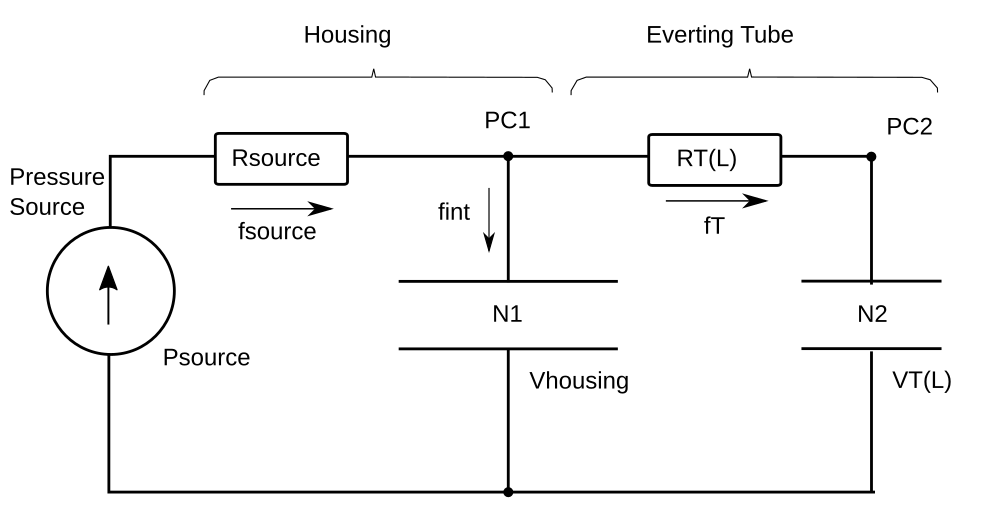
\includegraphics[width=.75\textwidth]{Figure_TwoCompartment.png}
\caption{Two compartment, lumped parameter model. }
\label{Fig:TwoCompartment}
\end{figure}

%  Use name of bibliography files without .bib extension
%\bibliography{brl}
\end{document}

